%!TEX root = ../report.tex
\documentclass[../report.tex]{subfiles}

\begin{document}
    \section{Background}
    \label{sec:background}

    % This is an optional section in which you can introduce concepts, terms, or methods that are important for understanding your approach and that would not directly fit in Sec. \ref{sec:methodology}.
    % If you do not need this section, comment out the respective line in \emph{report.tex}.
    \subsection{Explainable AI}
    Explainable AI (XAI) is a field of AI research that focuses on making AI systems more understandable and interpretable. It aims to provide explanations for AI model predictions, decisions, and behaviors, helping users understand how the model arrives at its conclusions. It can be grouped into three categories: post-hoc vs intrinsic, local vs global, model agnostic vs model specific explanations. Post-hoc explanations are generated after the model has been trained, while intrinsic explanations are built into the model architecture. Local explanations focus on explaining the model's decision for a specific input, while global explanations focus on explaining the model's behavior over a range of inputs. Model agnostic explanations are independent of the model architecture, while model specific explanations are specific to the model architecture  \cite{molnar2020interpretable}. 
    \subsection{Audio Waveform}
    An audio waveform represents the temporal evolution of sound pressure variations as a digital signal. It plots amplitude against time, where amplitude corresponds to the instantaneous sound pressure level. In digital form, the waveform consists of discrete samples captured at a fixed sampling rate, known as sampling. Sampling is the process of converting a continuous analog signal into a sequence of discrete numerical values by measuring the signal's amplitude at regular time intervals \cite{symons2013digital}. The sampling rate, measured in Hertz (Hz), determines how many samples are taken per second - for example, CD-quality audio uses 44.1 kHz sampling rate, meaning 44,100 samples are taken every second. While waveforms provide a complete representation of the audio signal, Automatic Speech Recognition (ASR) systems typically transform them into more compact features like spectrograms for efficient processing \cite{rabiner2007introduction}.
    \begin{figure}[ht]
        \centering
        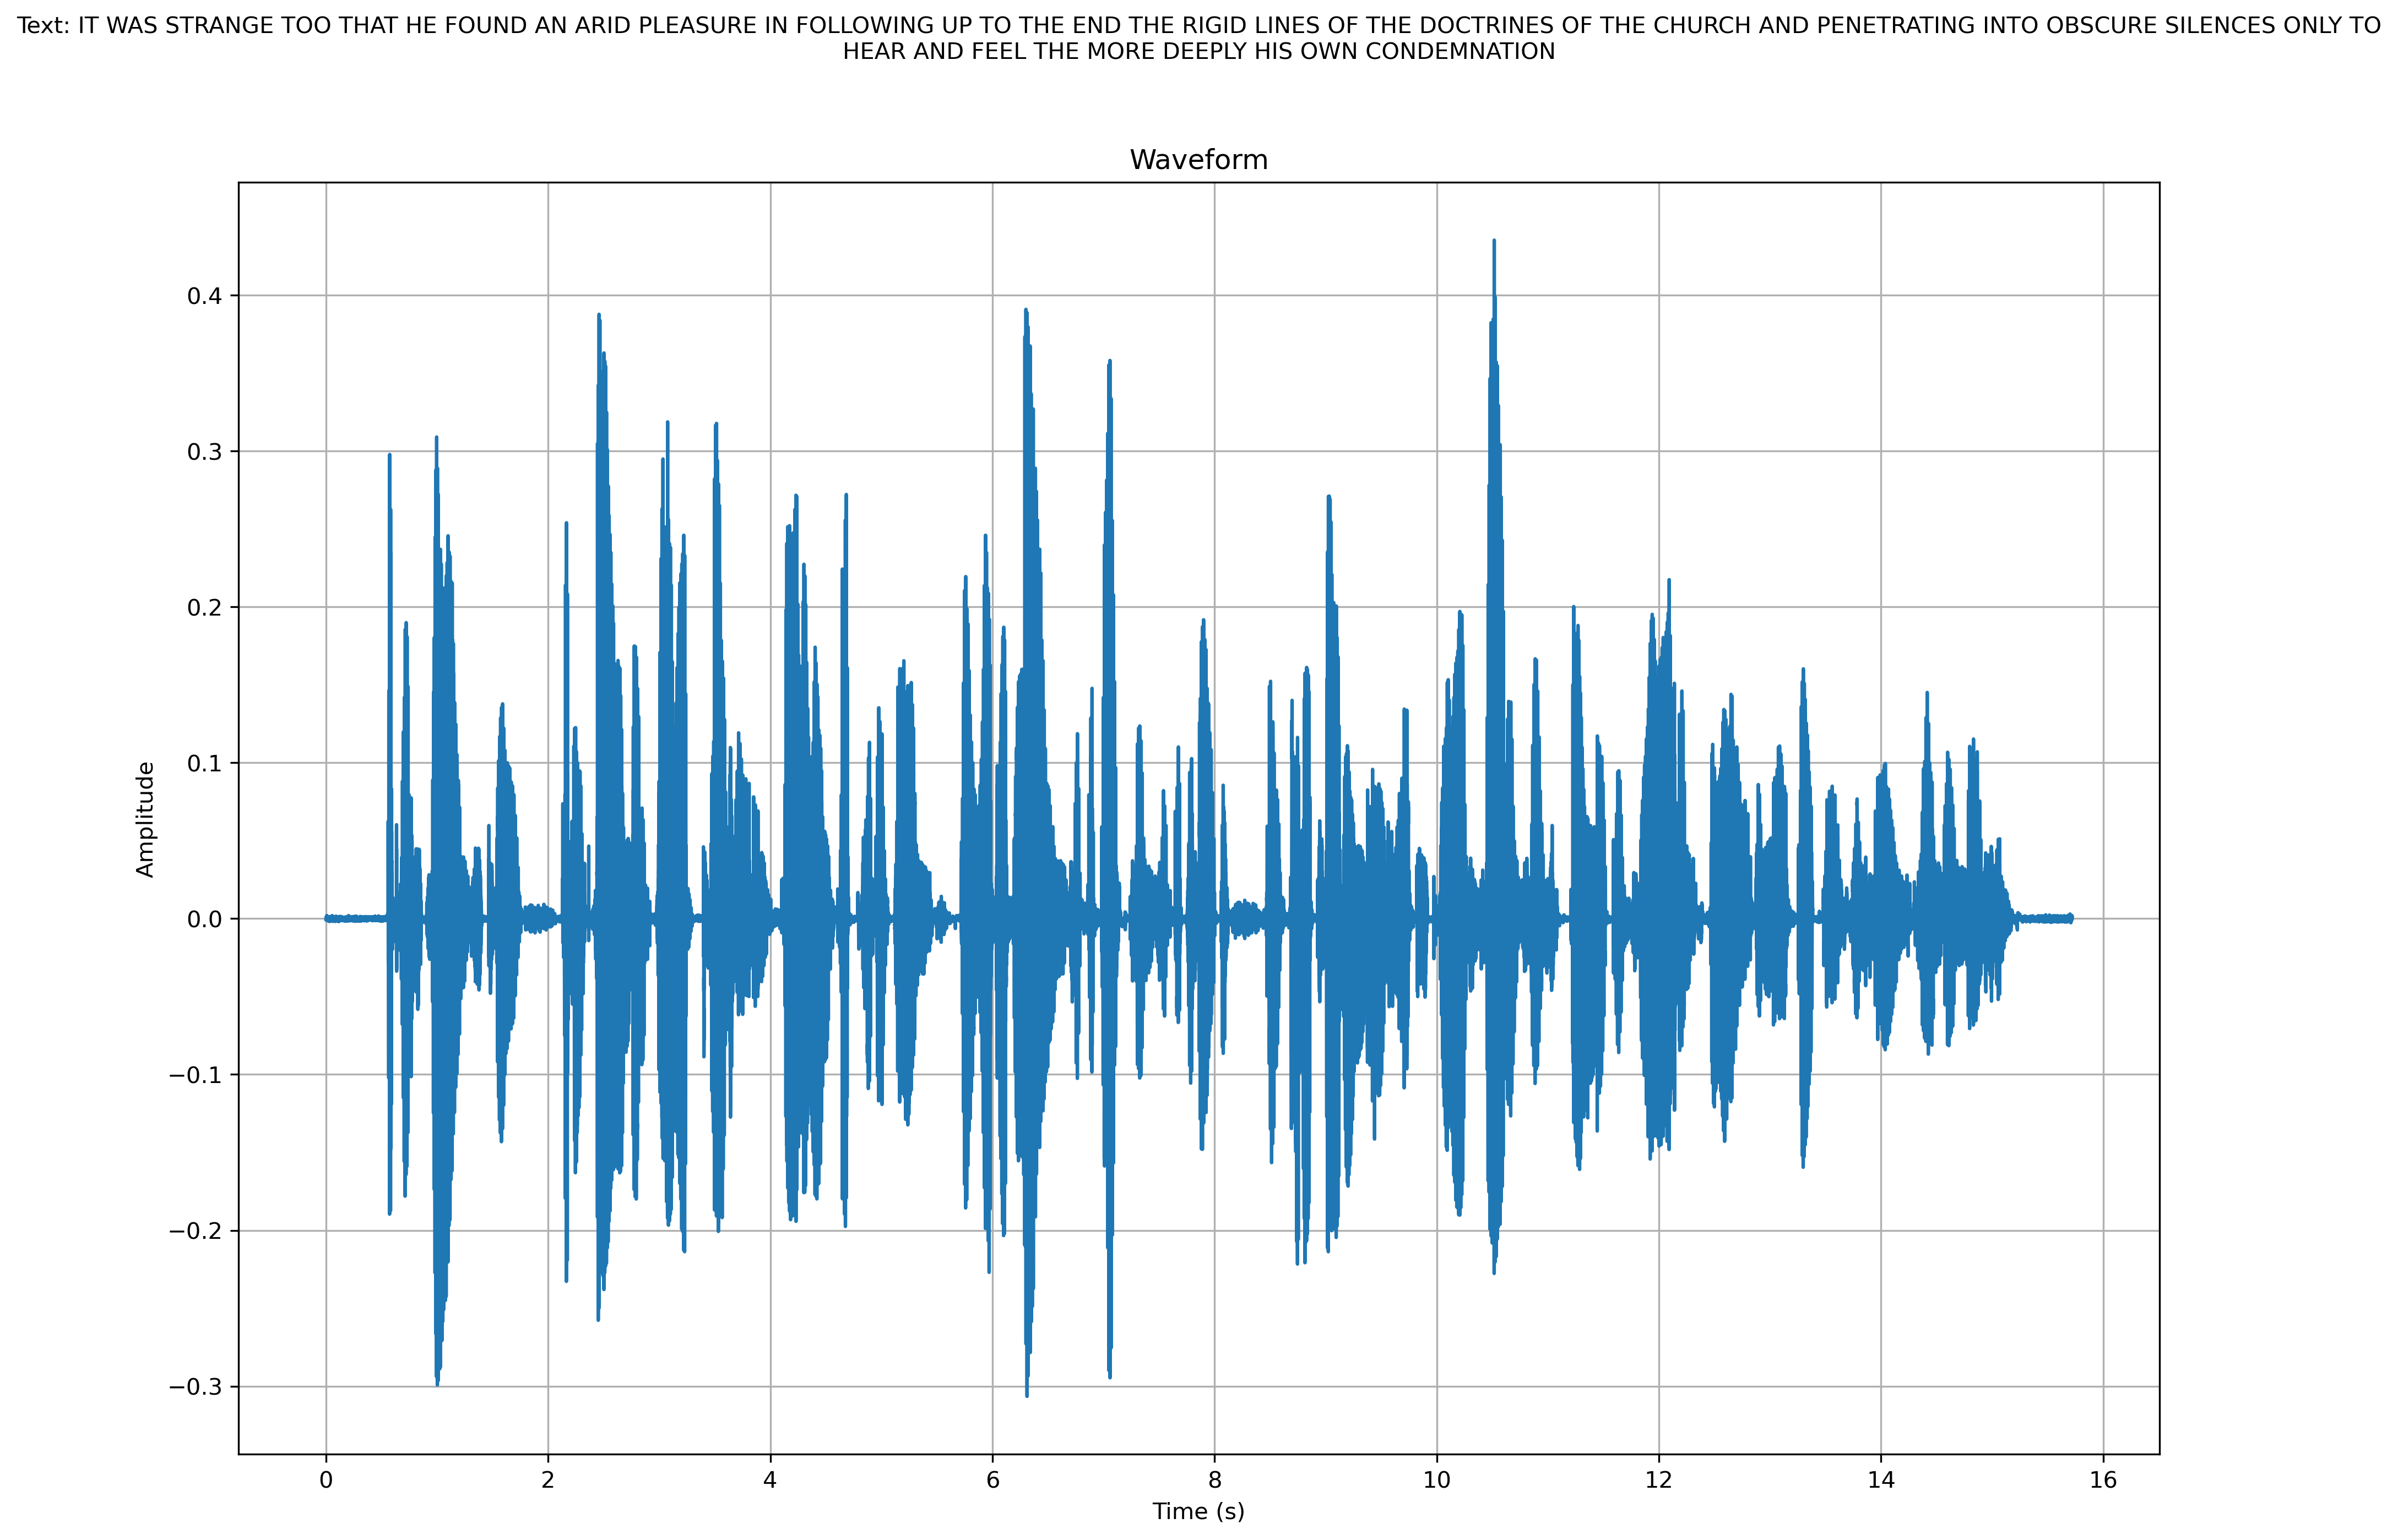
\includegraphics[width=0.8\linewidth]{../figures/waveform.png}
        \caption{Audio waveform of an example from LibriSpeech dataset}
        \label{fig:audio_waveform}
    \end{figure}
    
    \subsection{Log-Mel Spectrograms}
    A spectrogram is a visual representation of the spectrum of frequencies in a sound signal as they vary with time. It is created by applying a Short-Time Fourier Transform (STFT) to the audio signal, which breaks it down into its frequency components over short time windows.

    A Mel spectrogram is a type of spectrogram where the frequency axis is converted to the Mel scale, a perceptual scale of pitches designed to approximate the way humans perceive sound frequencies \cite{mel_scale}. It is based on the idea that humans do not perceive pitch linearly; instead, our perception of pitch is more closely related to a logarithmic scale. This transformation emphasizes frequencies that are more relevant to human perception, making it particularly useful for audio processing tasks. The Mel scale is approximately linear below 1 kHz and logarithmic above 1 kHz \cite{stanford_nlp_lecture}. The Mel filter bank consists of a series of overlapping triangular filters, each corresponding to a "Mel bin." Each Mel bin represents a range of frequencies, and the output of each filter is the sum of the energy in that frequency range. The number of Mel bins determines the resolution of the Mel spectrogram.

    The need for Log-Mel spectrograms arises from the fact that the human ear perceives loudness on a logarithmic scale. By taking the logarithm of the Mel spectrogram, we obtain a Log-Mel spectrogram, which better aligns with human auditory perception. This representation is particularly useful for ASR models as it captures the essential features of speech while reducing dimensionality.
    A Log-Mel spectrogram can be interpreted by examining its three main dimensions:
    \begin{itemize}
        \item The horizontal axis represents time progression
        \item The vertical axis shows frequency in Mel scale (emphasizing lower frequencies that are more relevant to human speech)
        \item Color intensity indicates the energy/amplitude at each time-frequency point, with brighter colors representing higher energy
    \end{itemize}
    
    In log-mel spectrograms, silent periods are visible as darker regions with minimal energy across frequencies, reflecting the absence of vocal activity. This visual pattern in spectrograms helps in distinguishing different phonetic elements and analyzing speech characteristics.
    
    \begin{figure}[ht]
        \centering
        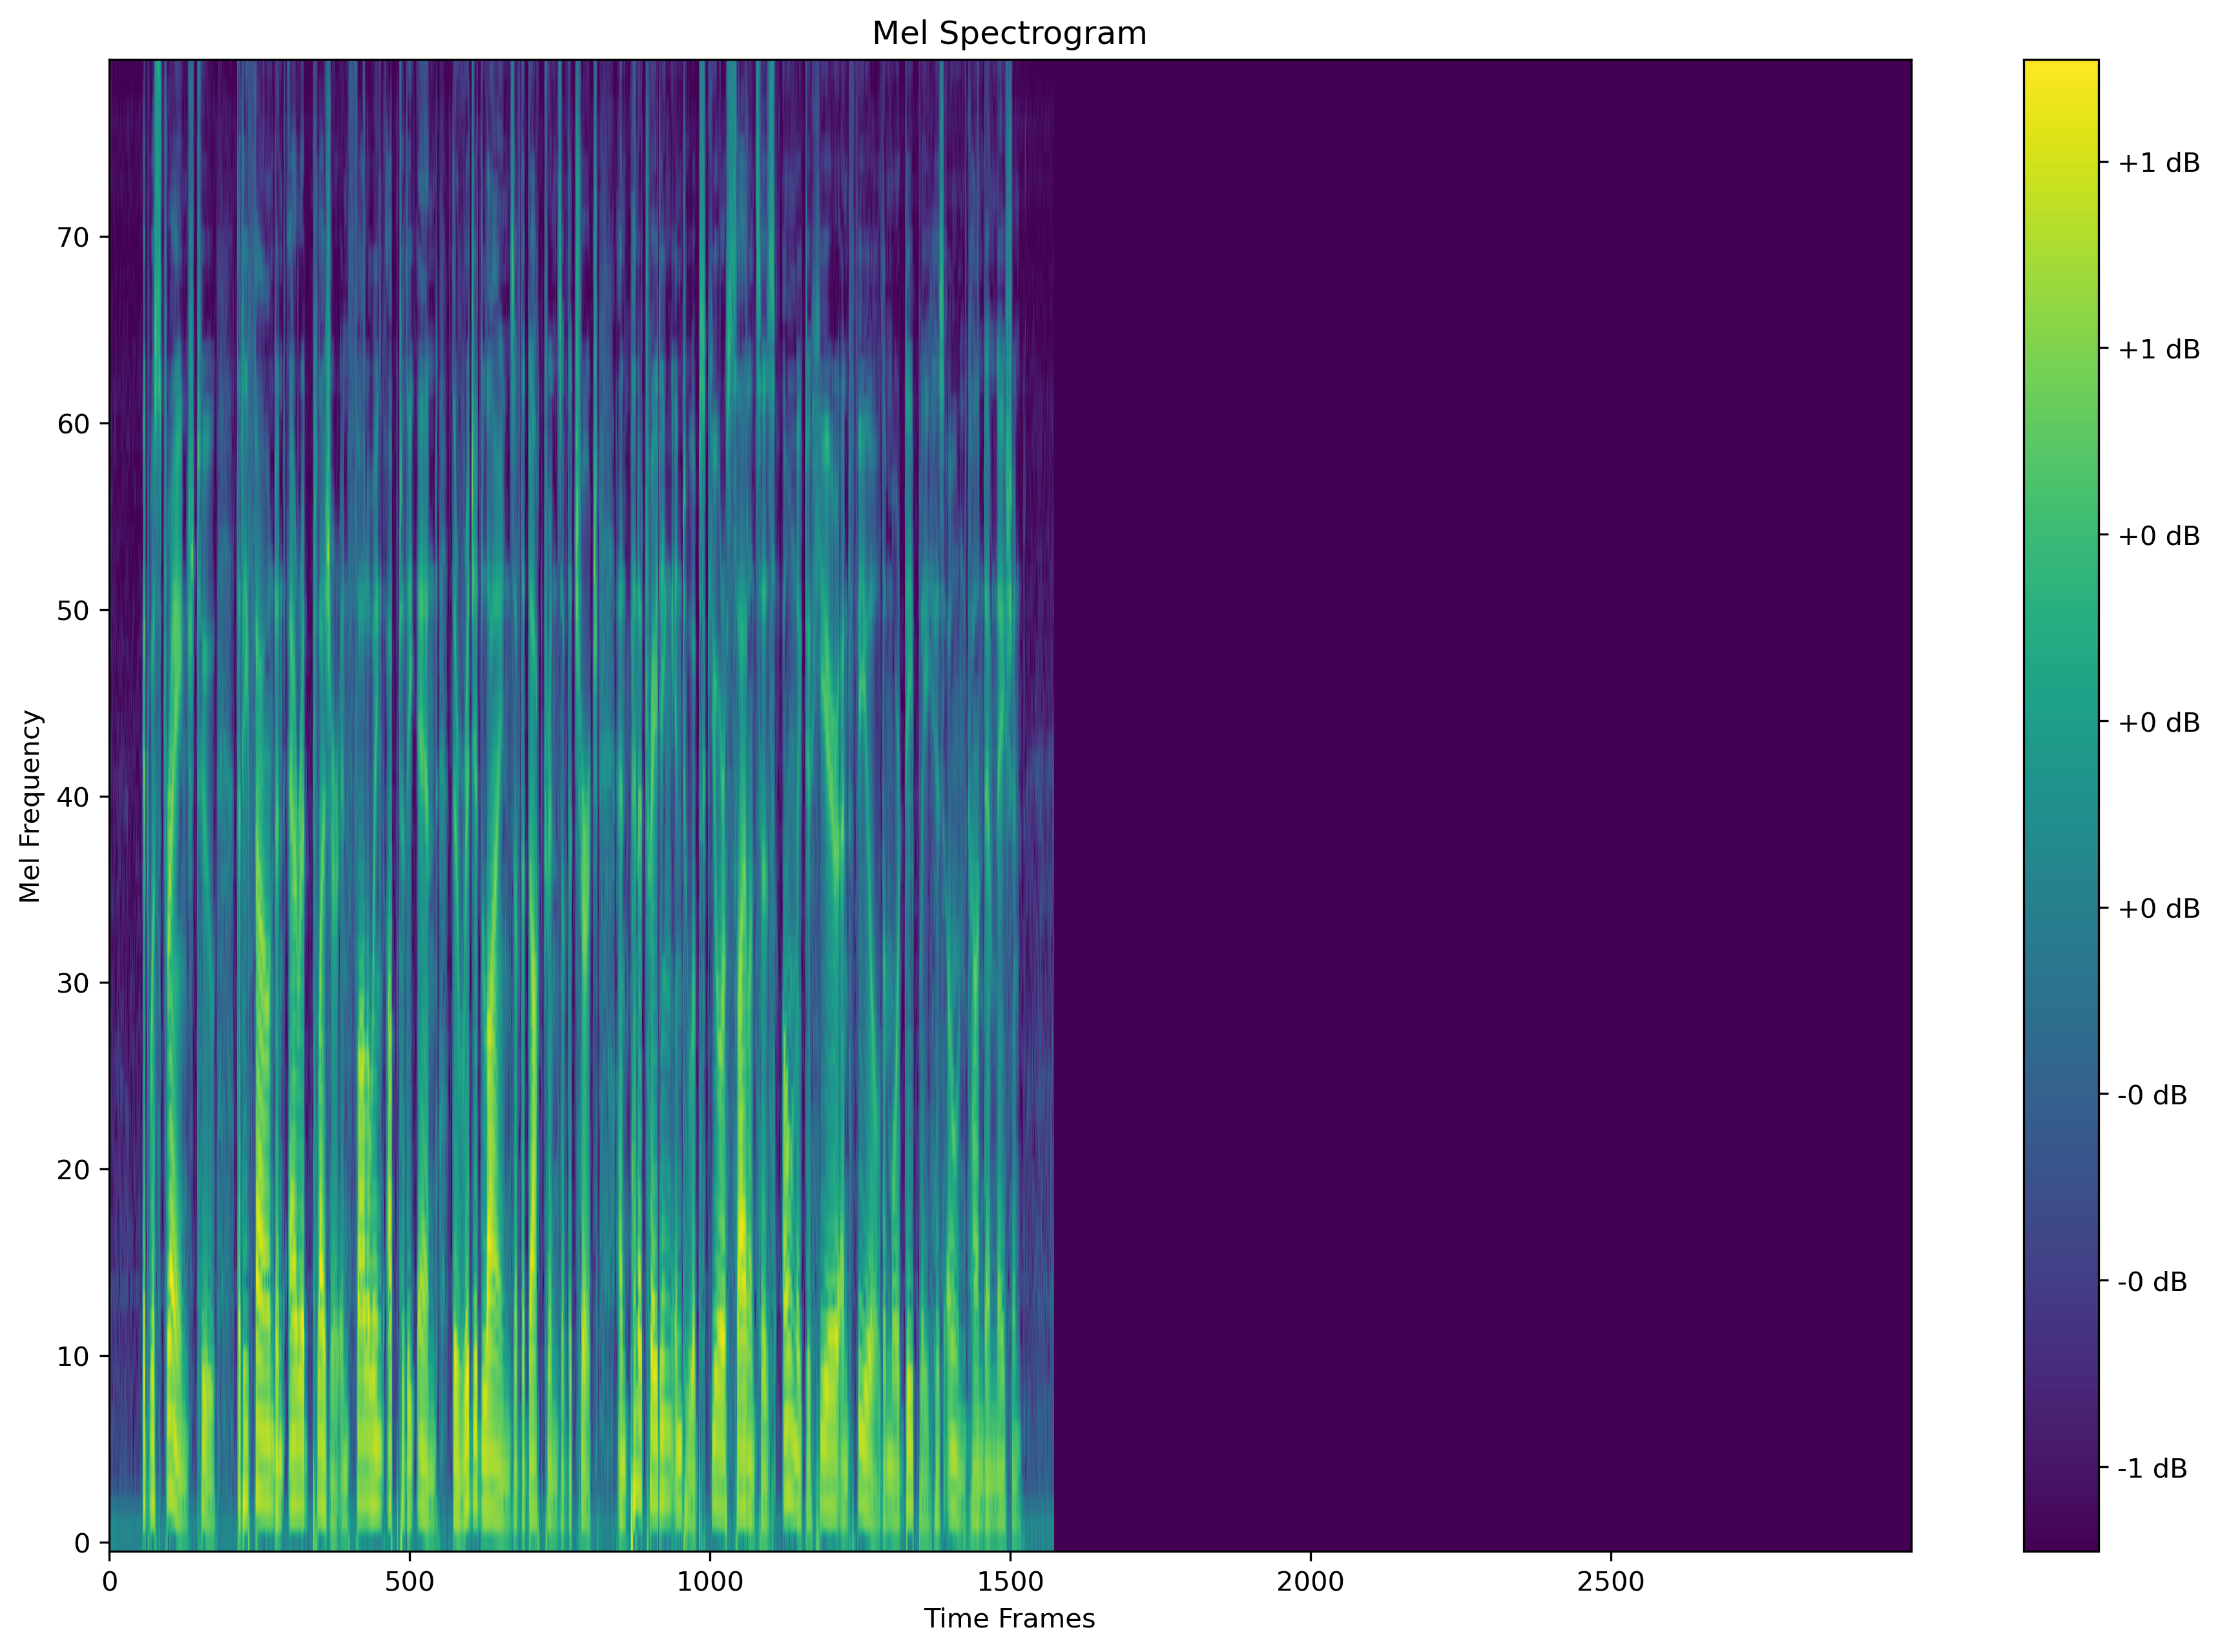
\includegraphics[width=0.8\linewidth]{../figures/mel_spectrogram.png}
        \caption{Log-Mel spectrogram with 80 mel bins}
        \label{fig:log_mel_spectrogram}
    \end{figure}

    \subsection{Attention Mechanisms}
    Attention mechanisms are integral to transformer models, a neural network architecture highly effective for sequence-to-sequence tasks such as Automatic Speech Recognition (ASR), as initially proposed by Vaswani et al. \cite{vaswani2017attention}. These mechanisms enable models to dynamically prioritize different segments of the input sequence, assigning varying importance to each token. In transformers, attention mechanisms facilitate the capture of long-range dependencies and contextual information, essential for interpreting complex input sequences like speech \cite{vaswani2017attention}.

    Each input token is transformed into three vectors: the query $Q$, the key $K$, and the value $V$. The query vector represents what information the token is looking for, the key vector represents what information the token contains that others might want to query, and the value vector contains the actual content that will be aggregated in the attention computation. These vectors are obtained by multiplying the input token embedding with learned weight matrices - trainable parameters that are optimized during model training to capture meaningful transformations of the input embeddings. The weight matrices start with random values and are gradually adjusted through backpropagation to learn optimal transformations for the specific task.

    \textbf{Operation:}
    \begin{itemize}
        \item \textbf{Self-Attention Mechanism:} In self-attention, the $Q$, $K$, and $V$ matrices are all derived from the same input sequence. This allows the model to focus on different parts of the sequence itself, capturing dependencies and relationships within the sequence.
        
        \item \textbf{Cross-Attention Mechanism:} In cross-attention, the $Q$ matrix comes from one sequence (e.g., the decoder in a transformer), while the $K$ and $V$ matrices come from another sequence (e.g., the encoder). This allows the model to focus on relevant parts of a different sequence, facilitating tasks like translation or multi-modal processing.
        
        \item \textbf{Attention Scores:} The attention scores are computed by taking the dot product of the query and key vectors, followed by a softmax function to normalize the scores. These scores determine how much attention each part of the input sequence receives.
        \begin{equation}
            \text{Attention}(Q, K, V) = \text{softmax}\left(\frac{QK^T}{\sqrt{d_k}}\right)V
            \label{eq:attention}
        \end{equation}
        where $d_k$ is the dimension of the key vectors. The scaling factor $\frac{1}{\sqrt{d_k}}$ prevents the dot products from growing too large in magnitude, which could push the softmax function into regions with extremely small gradients.
        \item \textbf{Output:} The final output of the attention mechanism is a weighted sum of the value vectors, where the weights are the attention scores. This output is then used in subsequent layers of the model to make predictions or generate outputs.
    \end{itemize}

    \subsection{Perturbations}
    Perturbations involve introducing small changes to the input data or model parameters to analyze their impact on the model's predictions. This technique is used in explainability methods to identify which parts of the input are most influential in the decision-making process, providing insights into the model's internal workings \cite{molnar2020interpretable}.

    \subsection{Cross Entropy Loss}
    Cross entropy loss is a common loss function used in classification tasks, including ASR. It measures the difference between the predicted probability distribution and the true distribution, penalizing incorrect predictions. Minimizing cross entropy loss helps improve the accuracy of the model's predictions \cite{pmlr-v202-mao23b, pmlr-v137-gordon-rodriguez20a}.

    The formula for cross entropy loss is:
    \begin{equation}
        L(y, \hat{y}) = -\sum_{i=1}^{N} y_i \log(\hat{y}_i)
        \label{eq:cross_entropy}
    \end{equation}
    where $y$ is the true distribution (often represented as a one-hot encoded vector), $\hat{y}$ is the predicted probability distribution, and $N$ is the number of classes.


    \subsection{Logits}
    In transformer models, logits are the raw output scores produced by the final linear layer before any normalization is applied. For ASR transformers particularly Whisper, these logits represent the model's pre-softmax predictions for each possible token (typically characters or subword units) in the vocabulary at each timestep. The logit values can be positive or negative and their magnitude indicates the model's confidence - larger values suggest stronger predictions for particular tokens.

    The logits are computed through a linear transformation of the final hidden states:
    \begin{equation}
        \text{logits} = W_{\text{vocab}} h + b
        \label{eq:logits}
    \end{equation}
    where $h$ is the hidden state vector from the final transformer layer, $W_{\text{vocab}}$ is a learned weight matrix that maps the hidden state dimension to the vocabulary size dimension (i.e., $W_{\text{vocab}} \in \mathbb{R}^{d_{\text{vocab}} \times d_{\text{model}}}$), and $b$ is a bias term, so logits are the size of the vocabulary for each forward pass of decoder while predicting the next token.

    These raw logits are then transformed into probabilities using the softmax function:
    \begin{equation}
        p(y_i) = \frac{\exp(\text{logit}_i)}{\sum_j \exp(\text{logit}_j)}
    \end{equation}
    where $p(y_i)$ is the probability of token $i$. This normalization ensures the probabilities sum to 1 while preserving the relative rankings of the logits \cite{bishop2006pattern}. In ASR systems, these probabilities guide the decoder in selecting the most likely transcription sequence \cite{radford2023robust}, and the logits are used to compute the cross entropy loss.

    \subsection{AtMan}
    As we explore multiple visual domain methods for explaining transformer based ASR models, we found AtMan by Deiseroth et al. \cite{NEURIPS2023_c83bc020} to be a promising method for our task, since it was modality agnostic. 
    It is a local explanation method that operates by perturbing the transformer's attention mechanism rather than the input space directly. Its core principle is to manipulate attention scores during the forward pass and observe how these manipulations affect the model's output logits at the decoder. Specifically, it suppresses attention to specific tokens (or groups of correlated tokens) and measures the resulting changes in the cross-entropy loss for target predictions. The magnitude of change in the output indicates the importance of the perturbed tokens for the specific prediction being explained. This approach is more efficient than traditional perturbation methods because it works in embedded token space rather than input space, and more memory-efficient than gradient-based methods since it only requires forward passes through the model instead of backpropagation. The method quantifies the influence of input tokens by comparing the model's original prediction with predictions under attention perturbation, effectively creating relevance maps that explain which parts of the input were most important for specific outputs.
    

\end{document}
